%%%%%%%%%%%%%%%%%%%%%%%%%%%%%%%%%%%%%%%%%
% Beamer Presentation
% LaTeX Template
% Version 1.0 (10/11/12)
%
% This template has been downloaded from:
% http://www.LaTeXTemplates.com
%
% License:
% CC BY-NC-SA 3.0 (http://creativecommons.org/licenses/by-nc-sa/3.0/)
%
%%%%%%%%%%%%%%%%%%%%%%%%%%%%%%%%%%%%%%%%%

%----------------------------------------------------------------------------------------
%	PACKAGES AND THEMES
%----------------------------------------------------------------------------------------

\documentclass[14pt,handout]{beamer}
%%\documentclass[14pt]{beamer}

\mode<presentation> {

% The Beamer class slide themes
\usetheme{Madrid} %i was using this one

% Beamer class color themes

%\usecolortheme{albatross}

%\setbeamertemplate{footline} % To remove the footer line in all slides uncomment this line
%\setbeamertemplate{footline}[page number] % To replace the footer line in all slides with a simple slide count uncomment this line

%\setbeamertemplate{navigation symbols}{} % To remove the navigation symbols from the bottom of all slides uncomment this line
}

\usepackage{graphicx} % Allows including images
\usepackage{booktabs} % Allows the use of \toprule, \midrule and \bottomrule in tables
\usepackage{hyperref}
\usepackage{helvet}
\usepackage[T1]{fontenc}
\usepackage{textcomp}

%----------------------------------------------------------------------------------------
%	TITLE PAGE
%----------------------------------------------------------------------------------------

\title[RNAseq Practical pt2]{RNAseq Analysis: A Practical Walkthrough (part 2/3)} % The short title appears at the bottom of every slide, the full title is only on the title page

\author{C. Ryan Campbell} % Your name
\institute[Duke] % Your institution as it will appear on the bottom of every slide, may be shorthand to save space
{
Duke University \\ % Your institution for the title page
\medskip
\textit{c.ryan.campbell@duke.edu} % Your email address
}
\date{26 Oct 2017} % Date, can be changed to a custom date

\begin{document}

\begin{frame}
\titlepage % Print the title page as the first slide
\end{frame}

\begin{frame}
\frametitle{Overview} % Table of contents slide, comment this block out to remove it
\tableofcontents % Throughout your presentation, if you choose to use \section{} and \subsection{} commands, these will automatically be printed on this slide as an overview of your presentation
\end{frame}

%----------------------------------------------------------------------------------------
%	PRESENTATION SLIDES
%----------------------------------------------------------------------------------------

%------------------------------------------------
\begin{frame}
\frametitle{Today's Goals}
\begin{itemize}
	\item<+-> Recap the workflow
	\item<+-> Discuss analyses
	\item<+-> Take the next analysis step
\end{itemize}
\end{frame}

%------------------------------------------------
\section{Workflow}
%------------------------------------------------

%------------------------------------------------
\begin{frame}
\frametitle{RNAseq Workflow}
\begin{enumerate}
	\large
	\item<+-> Get in your groups
	\item<+-> Recreate the diagram from two weeks ago
	\begin{itemize}
		\item<+-> Pick a step
		\item<+-> Fill in a description and software
		\item<+-> Should take about 10 minutes
	\end{itemize}
\end{enumerate}
\end{frame}

%%%------------------------------------------------
%%\begin{frame}
%%\frametitle{Group Guessing Game - No Phones!}
%%\begin{itemize}
%%	\item<+-> How tall, in feet, is Duke Chapel?
%%	\item<+-> How many people does it hold?
%%	\item<+-> What year was it completed?
%%	\item<+-> Your answer = 10 * height + capacity + year completed
%%\end{itemize}
%%\end{frame}

%------------------------------------------------
%%\begin{frame}
%%\frametitle{Group Guessing Game - No Phones!}
%%\begin{itemize}
%%	\item<+-> Your answer = 10 * height + capacity + year completed
%%	\item<+-> Work with your group to guess the number and write it and your name on a piece of paper
%%	\item<+-> The most accurate guess will get first pick of which section to describe
%%	\item<+-> Make your guesses now, you have 2 minutes
%%\end{itemize}
%%\end{frame}

%------------------------------------------------
%%\begin{frame}
%%\frametitle{The Answer...}
%%\begin{itemize}
%%	\item<+-> is 210 feet, 1800 occupants, completed in 1932
%%	\item<+-> (210 * 10) + 1800 + 1932 = 5832
%%	\item<+-> Pick which section you'd like to recap
%%	\begin{enumerate}
%%		\item<+-> Library Prep
%%		\item<+-> Sequencing
%%		\item<+-> Quality Check Data
%%		\item<+-> Trim Data
%%		\item<+-> Align
%%	\end{enumerate}
%%	\item<+-> Recap - input, output, software
%%\end{itemize}
%%\end{frame}

%------------------------------------------------
\begin{frame}
\frametitle{RNAseq Workflow}
\begin{enumerate}
	\large
	\item<+-> Get in your groups
	\item<+-> Recreate the diagram from two weeks ago
	\begin{itemize}
		\item<+-> Pick a step
		\item<+-> Fill in a description and software
		\item<+-> Should take about 10 minutes
	\end{itemize}
\end{enumerate}
\end{frame}

%------------------------------------------------
\begin{frame}
\frametitle{slogin OR sbatch script}
\begin{itemize}
	\large
	\item<+-> Refresher: What is the difference?
	\item<+-> Make sure you're making a conscious choice between the two
	\item[] 
	\item<+-> When you analyze your files, make sure to use an sbatch script
\end{itemize}
\end{frame}

%------------------------------------------------
\begin{frame}
\frametitle{slogin OR laptop}
\begin{itemize}
	\large
	\item<+-> What is the difference?
	\item<+-> Which processes will go where?
	\item[]
	\item<+-> What are the strengths and weaknesses of each?
\end{itemize}
\end{frame}

%------------------------------------------------
\begin{frame}
\frametitle{SLURM Interactive Node}
\begin{itemize}
	\item Later we'll be troubleshooting \texttt{htseq-count}
	\item For that you should use an ``interactive node''
	\item This runs like a sbatch job, but it appears as a terminal that you can interact with
	\footnotesize
	\ttfamily
	\begin{block}{}
	\item[] srun --mem-per-cpu=16000MB --pty bash -i
	\end{block}
	\sffamily
	\item You've just requested a 16GB (powerful laptop) size node on SLURM
\end{itemize}
\end{frame}

%------------------------------------------------
\section{tophat Output}
%------------------------------------------------

%------------------------------------------------
\begin{frame}
\frametitle{tophat Output}
\begin{itemize}
	\item<+-> tophat - alignment software
	\item<+-> What (in english) is that doing?
	\item<+-> What is the output file type?
\end{itemize}
\end{frame}

%------------------------------------------------
\begin{frame}
\frametitle{tophat bam files}
\begin{itemize}
	\item<+-> tophat output = bam file
	\item<+-> fastq data aligned to your genome
	\item<+-> How many bam files should you have per treament/condition?
	\item<+-> IGV can be used to ``check'' the bam
\end{itemize}
\end{frame}

%------------------------------------------------
\section{Counting \& Analysis}
%------------------------------------------------

%------------------------------------------------
\begin{frame}
\frametitle{Counting \& Analysis}
\begin{itemize}
	\item<+-> Now that we have bam files the next step is to count the reads
	\item<+-> And using those counts compare gene expression levels
	\item<+-> We'll be using HTseq and DeSeq2
\end{itemize}
\end{frame}

%------------------------------------------------
\subsection{Software Options}
%------------------------------------------------

%------------------------------------------------
\begin{frame}
\frametitle{Software Options}
\begin{itemize}
	\item<+-> There are many options for counting and analysis
	\item<+-> cufflinks (cuffdiff/cuffcompare/etc) is popular
	\item<+-> HTSeq and DESeq2 are more straightforward
	\item<+-> DESeq2 gets us into R quicker
	\item<+-> (thus my decision to use them for the tutorial)
\end{itemize}
\end{frame}

%------------------------------------------------
\begin{frame}
\frametitle{HTSeq}
\begin{itemize}
	\item<+-> python-based program to count reads
	\item<+-> Input: 
%%	\item<+-> .bam file and .gtf/.gff
	\item<+-> Output:
%%	\item<+->  A table of counts by gene
\end{itemize}
\end{frame}

%------------------------------------------------
\begin{frame}
\frametitle{DESeq2}
\begin{itemize}
	\item<+-> R-based program to analyze expression
	\item<+-> Input: 
%%	\item<+-> A table of counts by gene
	\item<+-> Output: 
%%	\item<+-> Graphs and (hopefully) Answers!!!
\end{itemize}
\end{frame}

%------------------------------------------------
\section{Tutorial}
%------------------------------------------------

%------------------------------------------------
\begin{frame}
\frametitle{Files to Use}
\begin{itemize}
	\item I've set up some example files to use for this tutorial
	\item They're human RNAseq files from a hypoxia experiment:
	\footnotesize
	\ttfamily
	\begin{block}{}
	\item[] ls -lthr /work/cc216/490S/cc216/RNAseq\_pt2
	\end{block}
	\sffamily
	\item What do you see? Which will you use?
\end{itemize}
\end{frame}

%------------------------------------------------
\begin{frame}
\frametitle{Files to Use}
\begin{itemize}
	\footnotesize
	\ttfamily
	\begin{block}{}
	\item[] ls -lthr /work/cc216/490S/cc216/RNAseq\_pt2
	\end{block}
	\begin{center}
		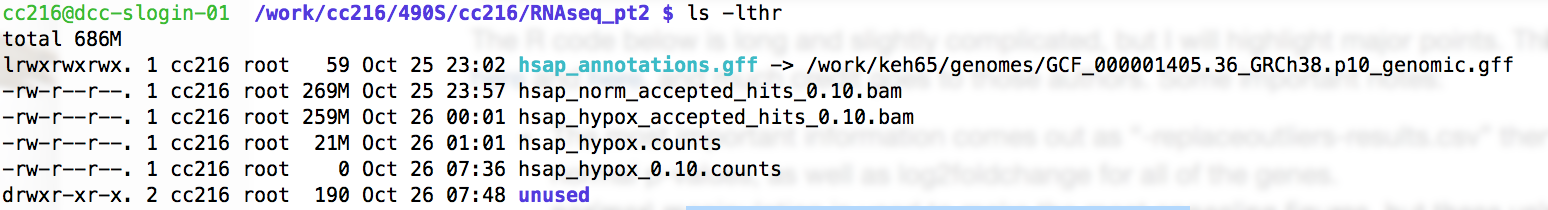
\includegraphics[width=.9\textwidth]{images_20171026_usefiles.png}
	\end{center}
\end{itemize}
\end{frame}

%------------------------------------------------
\subsection{HTSeq}
%------------------------------------------------

%------------------------------------------------
\begin{frame}
\frametitle{htseq-count}
\begin{itemize}
	\item We'll be using htseq-count
	\item This will count the number of reads mapped to each gene
	\item That data will be taken into DESeq2
	\footnotesize
	\ttfamily
	\begin{block}{}
	\item[] /opt/apps/rhel7/Python-2.7.11/bin/htseq-count 
	\end{block}
	\sffamily
	\item[] (go ahead and put it in your path)
\end{itemize}
\end{frame}

%------------------------------------------------
\begin{frame}
\frametitle{SLURM Interactive Node}
\begin{itemize}
	\item Now that we're about to troubleshoot \texttt{htseq-count} hopefully your SLURM node is open
	\footnotesize
	\ttfamily
	\begin{block}{}
	\item[] srun --mem-per-cpu=16000MB --pty bash -i
	\end{block}
	\sffamily
\end{itemize}
\end{frame}

%------------------------------------------------
\begin{frame}
\frametitle{htseq-count}
\begin{itemize}
	\item What does HTSeq do?
	\item What are its flags and options?
	\footnotesize
	\ttfamily
	\begin{block}{}
	\item[] htseq-count <options> <alignment bam> <gff file> > <count output>
	\end{block}
	\sffamily
	\item Probably important: -f, -s, -t
\end{itemize}
\end{frame}

%------------------------------------------------
%%\begin{frame}
%%\frametitle{htseq-count}
%%\begin{itemize}
%%	\item Here are the flags that I got it to work with:
%%	\footnotesize
%%	\ttfamily
%%	\begin{block}{}
%%	\item[] htseq-count -s no -r pos -t exon -i gene -f bam hsap\_hypox\_accepted\_hits\_0.10.bam hsap\_annotations.gff > hsap\_hypox\_0.10.counts
%%	\end{block}
%%	\sffamily
%%\end{itemize}
%%\end{frame}

%------------------------------------------------
\subsection{DESeq2}
%------------------------------------------------

%------------------------------------------------
\begin{frame}
\frametitle{DESeq2}
\begin{itemize}
	\item<+-> What does DESeq2 do?
%%	\item<+-> Compares the count matrices from many samples
	\item<+-> Where do you run it?
%%	\item<+-> In R on your laptop
\end{itemize}
\end{frame}

%------------------------------------------------
\begin{frame}
\frametitle{DESeq2 guides}
\begin{itemize}
	\item<+-> We'll get into DESeq2 next week
	\item<+-> If you want to get started here are some guides:
	\item<+-> \href{http://bioconductor.org/packages/devel/bioc/vignettes/DESeq2/inst/doc/DESeq2.html}{Walkthrough}
	\item<+-> \href{https://www.bioconductor.org/packages/release/bioc/html/DESeq2.html}{Bioconductor Manual} 
	\item<+-> \href{https://www.bioconductor.org/help/workflows/rnaseqGene/}{Bioconductor Walkthrough}
\end{itemize}
\end{frame}


%------------------------------------------------
\begin{frame}
\Huge{\centerline{The End}}
\end{frame}

%----------------------------------------------------------------------------------------

\end{document} 